\section{问题一：场景 A 的两种切图与调度方案}
两种求解方案均面向场景 A：跨子图张量经共享 DDR 中转，私有缓存不跨 Task 保留。方案一以结构感知初解和受保护的有限评价机会控制计算成本；方案二扩大结构候选覆盖，再用官方模拟筛选并局部改进。两者共享目标函数与可行域，差别发生在候选生成、任务放置和搜索资源分配，而非硬件假设。以下先建立共同模型，再分别讨论算法，最后在相同单核基准下比较五核结果。
\subsection{场景 A 的共同组合优化模型}
令 $V_c$ 为所有非 COPY 算子。映射 $\pi$ 把它们恰好分配给 $q$ 个非空子图，$m$ 把每个子图分配给一个核心，$\sigma_c$ 给出核心 $c$ 上各子图的顺序。把跨子图的数据前驱构成商图，再加入每核顺序边，所得扩展商图必须无环；否则即使原图无环，核心顺序仍可能与跨核等待构成死锁。合法方案集合记为 $\mathcal P_A(k)$。对于每份方案，官方内层启发式先产生实际 COPY 和核内 Pipe 序，再进行共享 DDR 事件仿真。我们以此可计算但不便线性化的函数定义目标：
\begin{equation}\label{eq:q1-objective}
\min_{p\in\mathcal P_A(k)}
\operatorname{lex}\left(T_i^A(p),D_i(p)\right),\qquad
T_i^A(p)=\max_{u\in\mathcal T(p)}f_u .
\end{equation}
这里的字典序表示优先缩短最后一个 Task 的完成时间；仅在周期相同时比较额外搬运。它是算法的选优规则，不把较少搬运误说成必然较短的周期。

Task $v$ 的开始须满足所有数据前驱释放和同核前一 Task 的间隔。以 $F_u$ 表示前驱完成时刻，$P_c(v)$ 表示核心 $c$ 上的前一 Task，可写为
\begin{equation}\label{eq:q1-release}
R_v \ge \max_{u\in\operatorname{pred}(v)}
\left(F_u+1000\,\mathbf 1\{m_u\ne m_v\}\right),\qquad
R_v\ge F_{P_{m_v}(v)}+100 .
\end{equation}
同核依赖不额外施加跨核的 $1000$ 周期，但跨 Task 张量仍须由 DDR 中转。公式\eqref{eq:q1-release}仅描述释放约束，不能单独算出时长；Cube、Vector、搬运 Pipe 的先后关系、L1/UB 溢出以及同时在途的 DDR 传输会改变 $F_u$。实际评价必须采用题目给出的事件过程。

为了识别一份输入被多个子图重复读取的情形，我们把共享张量与多个消费算子的关系视为有向超边，保留原图方向和商图无环性。多层次无环划分研究说明，此类表示比仅统计两两割边更适合描述共享输入\cite{popp}。我们借鉴这一表示和粗化思想，但没有照搬其平衡目标或宣称实现了文献的完整算法；本题的最终目标仍是式\eqref{eq:q1-objective}。

\subsection{场景 A 的物理语义与可行性}
场景 A 中子图与 Task 一一对应，即 $\mathcal T(p)=\{V_1,\ldots,V_q\}$。两个 Task 即使被映射到同一个核心，前者的私有 L1/UB 状态也不能跨 Task 保留；跨子图张量必须先写至 DDR，后继 Task 再读回。因此子图边界上的数据路径由 $\pi$ 决定，核心映射 $m$ 并不能把同核边界通信改成免费的片上读取。这一点与场景 B 是根本区别。核心 $c$ 上按 $\sigma_c$ 串行执行的 Task 之间另有固定的 $100$ 周期切换间隔；跨核数据前驱给目标 Task 施加 $1000$ 周期等待。若有多个前驱，目标 Task 等到\emph{最后一个}约束满足即可，而非把所有前驱延迟相加。

将 Task $r$ 的实际开始、完成记为 $S_r,F_r$，其数据前驱集合为 $\operatorname{Pred}_{\pi}(r)$。若 $a\prec_c r$ 表示核心 $c=m(r)$ 上排在 $r$ 前面的最后一个 Task，释放规则可写为
\begin{align}\label{eq:q1-release-expanded}
S_r&\ge \max_{a\in\operatorname{Pred}_\pi(r)}
  \{F_a+\delta_{ar}\},&
\delta_{ar}&=1000\,\mathbf 1\{m(a)\ne m(r)\},\\
S_r&\ge F_{\operatorname{prev}_{\sigma_c}(r)}+100
&&\text{若该前一 Task 存在}.\nonumber
\end{align}
式\eqref{eq:q1-release-expanded}只描述外层 Task 的可发射时刻。某 Task 的 $F_r-S_r$ 并非常数：展开出的四条 Pipe 上的操作依赖、共享 DDR 竞争以及 L1/UB 压力都会影响它。优化器因此必须先给出合法 $(\pi,m,\sigma)$，再调用官方核内与多核评价过程得到真实 $F_r$。若仅用一个预先标定的“子图长度”代入普通列表调度，便会在两个候选改变 DDR 发射重叠时给出相同预测，却可能得到不同的正式完成时间。

四条 Pipe 分别执行矩阵运算、向量运算和两类搬运。用 $P(e)$ 表示事件 $e$ 所属 Pipe，核内候选排程给每条 Pipe 一个确定顺序。对相同核心及相同 Pipe 的前后事件有 $f_{\operatorname{prevPipe}(e)}\le s_e$；跨 Pipe 只由真实算子依赖与内存复用依赖约束，不人为强制串行。对任一私有存储池 $r\in\{\mathrm{L1},\mathrm{UB}\}$，展开后的物理驻留集合 $\mathcal R_{c,r}(t)$ 必须满足
\begin{equation}\label{eq:q1-capacity}
\sum_{x\in\mathcal R_{c,r}(t)} b_x\le C_r,\quad
C_{\mathrm{L1}}=524288,\quad C_{\mathrm{UB}}=131072
\qquad(\forall c,t).
\end{equation}
如果未经换出换入就会越界，官方核内启发式会引入附加搬运来维持容量合法。因而式\eqref{eq:q1-capacity}约束的是\emph{实际展开的执行}，不能把“候选静态张量大小总和未超限”误认为充分条件，也不能把溢出惩罚写成只由子图算子数量决定的固定函数。

\subsection{额外搬运的计数口径}
令 $B_{\rm all}(p)$ 为官方展开方案在 DDR 上的总逻辑 COPY 字节数，$B_{\rm orig}$ 为未切图输入中已经要求的基础 COPY 字节数。题目所报的额外搬运定义为
\begin{equation}\label{eq:q1-added-bytes}
D(p)=B_{\rm all}(p)-B_{\rm orig}.
\end{equation}
这个定义覆盖了子图边界传递、原始输入的重复读取，以及核内启发式因容量不足插入的换入换出。正文始终用式\eqref{eq:q1-added-bytes}与官方输出核对，而不用简单割边权和代替它。设输入张量 $x$ 被 $r_x(\pi)$ 个不同 Task 消费，则在独立 Task 都需要从 DDR 读入这一语义下，\emph{相对一次读取}的重复输入字节可用
\begin{equation}\label{eq:q1-duplicate-input}
D_{\rm input}^{\rm proxy}(\pi)=
\sum_{x\in\mathcal X_{\rm input}}\bigl(r_x(\pi)-1\bigr)_+\,b_x
\end{equation}
作静态代理。它反映多消费超边的割开程度：同一张量的三个消费者分处三个 Task 时，不宜只看三条两两边的权重；若三个消费者聚在一个 Task，代理重复读入为零。但式\eqref{eq:q1-duplicate-input}只涉及外部输入的一个组成项，不能再把同一张量的边界读入重复加进另一个“割边项”以免双计。中间张量的写出次数、各目标 Task 的读取及真实溢出，由官方展开后的事件记录裁决。

减少 $D(p)$ 并不等价于减少 $T(p)$。反例是合并两个可并行子图：该动作可能删除边界 COPY，却使原来可分别运行的矩阵链和向量链被一个 Task 的内部顺序或容量压力拖慢。反过来，少量额外搬运若释放关键任务的并行空间，也可能缩短 Makespan。因此式\eqref{eq:q1-objective}采用完成时间优先的字典序；并在结果章节同时报告 $D(p)$ 的变化，而不预设它必与主目标同向。

\subsection{方案条件下的下界及其推导}
共同计算下界 $L_0(k)$ 已由式\eqref{eq:universal-compute-bound}给出。场景 A 还允许对固定方案 $p$ 构造更贴近其 Task 结构的事后下界。令 $W_{M,r}=\sum_{e\in V_r\cap O_M}c_e$，$W_{V,r}=\sum_{e\in V_r\cap O_V}c_e$；同一 Task 内这两类 Pipe 可以重叠，却各自不能在本 Pipe 上并发，因此
\begin{equation}\label{eq:q1-task-min-duration}
F_r-S_r\ge \underline\tau_r:=\max\{W_{M,r},W_{V,r}\}.
\end{equation}
若核心 $c$ 上有 $n_c$ 个 Task，则该核从第一个 Task 起始到最后一个 Task 完成至少占用 $\sum_{r:m(r)=c}\underline\tau_r+100(n_c-1)_+$ 周期。令 $\mathcal P(H(p))$ 为扩展商图的路径集合，在路径 $(r_1,\ldots,r_h)$ 上，每个任务的最短计算时间和依赖释放必须依次经过。因此
\begin{align}\label{eq:q1-fixed-plan-lb}
T(p)\ge L_A(p):=\max\Bigg\{&
L_0(k),\ \frac{B_D(p)}{60},\
\max_c\bigg[\sum_{r:m(r)=c}\underline\tau_r+100(n_c-1)_+\bigg],\\
&\max_{(r_1,\ldots,r_h)\in\mathcal P(H(p))}
\bigg[\sum_{j=1}^{h}\underline\tau_{r_j}
+\sum_{j=1}^{h-1}\underline\delta(r_j,r_{j+1})\bigg]\Bigg\}.\nonumber
\end{align}
对路径中的数据依赖弧，跨核时取 $\underline\delta=1000$，同核时至少为 $100$ 的任务间隔；对纯顺序弧，只取 $100$。若一对任务既有数据依赖又有顺序关系，同一间隔仅计一次。式\eqref{eq:q1-fixed-plan-lb}的每项分别由计算工作、带宽容量、同核串行和依赖链推出，取最大而不是相加，避免把可重叠资源时间重复计算。

这个界是\emph{针对所选划分和映射的条件界}。例如合并任务会改变 $B_D(p)$、$n_c$ 和路径集；把方案 $p_1$ 的 $L_A(p_1)$ 当作方案 $p_2$ 的最优下界没有依据。我们用它寻找当前方案的主导限制：若同核负载项远大于其他项，优先考虑拆分或迁核；若关键路径项主导，优先处理路径上的边界与核心切换；若带宽项主导，检查重复输入及边界流量。这是一条有物理解释的候选分配规则，不是由下界直接求得最优划分。

\subsection{合并与拆分的边际判断}
考虑相邻子图 $A,B$ 与一份大小为 $b$ 的边界张量。若把它们合成同一 Task，理论上可删除这份边界上的部分 DDR 事件与释放等待；但这份“被删除的字节数”不一定等于 $b$ 或 $2b$，因为还取决于共享消费者、输出写回以及已有 COPY。令 $\Delta B_{\rm boundary}$ 为按场景 A 展开规则实际消失的边界字节，$\Delta B_{\rm spill}$ 为合并后新增的溢出字节。一个\emph{仅用于排序}的净搬运近似为
\begin{equation}\label{eq:q1-merge-traffic-proxy}
\widehat{\Delta B}
=\Delta B_{\rm boundary}-\Delta B_{\rm spill}.
\end{equation}
若合并删除一个实际落在关键链上的跨核 Task 边，还可能减少 $1000$ 周期释放；若删除的是同核相邻 Task 边，最多直接省下该处 $100$ 周期间隔。然而被删除的等待与传输可以重叠，也可能原本根本不控制最终输出，所以不能把 $\Delta B_{\rm boundary}/60+1000$ 作为\emph{必得}的 Makespan 改善。真正的差值为
\begin{equation}\label{eq:q1-merge-exact}
\Delta T_{\rm merge}
=T^A(p_{\rm old})-T^A(p_{\rm merged}),
\end{equation}
只能在两个完整方案通过官方评估后确定。式\eqref{eq:q1-merge-traffic-proxy}给出有依据的候选顺序，式\eqref{eq:q1-merge-exact}才给出是否接受的结论。拆分动作同理：它增加边界开销，却可能降低单核长尾与局部溢出。固定算子个数切块无法表达这种结构差异，故初始划分同时覆盖整分量与少量主导分量拆分。

\subsection{方案一：结构感知初解与有界搜索}
首先构造整图保底方案与依赖贪心方案。对没有计算依赖的弱连通分量，尝试保持完整并按估计的最长 Pipe 工作量分核；这样能释放天然并行度，且减少不必要的分量内切边。若一个主导分量明显压过其余分量，则在满足无环性的拓扑窗口中有限拆分，以免完整保留造成单核长尾。共享输入复用、局部核内时长和容量压力同时参与候选排序；局部估计只负责提出方案，不能替代官方全局仿真。

将候选子图调度到核心时，先按后续关键工作量排序，再为每个子图寻找最早合法插入空隙和预计完成时间较小的核心。该思想与最早完成时间列表调度相近\cite{topcuoglu}，但本题必须附加式\eqref{eq:q1-release}、共享 DDR 和真实容量条件。随后在固定的评价机会内，尝试少量关键区域的边界调整、核心迁移与顺序修复；每个被提出的完整方案均检查操作覆盖和扩展商图无环，并由原始评价语义选优。

当前采用方案对每个多核配置限制为 $12$ 次评价机会、确定性种子 $0$。基础粒度搜索保留机会，结构新候选须通过事件成本准入；失败的候选不能因预测好就替代实测较优方案。当前研究版本启用了局部成本、关键路径、一般映射空隙插入、通信排序、划分保护、共享输入及有限区域修复。实验中测试过而未被采用的事件池整体重排序、扩大的自适应组合等，不计入本轮主结果。固定预算使评价调用数随图数线性增长；候选构造与图规模相关，但不枚举指数数量的分组、映射和任务排列。

\subsubsection{初解生成的结构依据}
求解先利用计算图的弱连通分量。两个互不相连的分量之间没有计算数据前驱；若把完整分量分别放到不同核心，不会产生分量间新的中间张量通信，因此它们是低成本的并行初解。设分量 $C$ 的矩阵、向量工作量分别为 $W_M(C),W_V(C)$，并定义两管道负载向量 $\mathbf w(C)=(W_M(C),W_V(C))$。若某分量的某项工作量超过平均每核份额，
\begin{equation}\label{eq:q1-dominant-component}
W_M(C)>\frac{W_M}{k}
\quad\text{或}\quad
W_V(C)>\frac{W_V}{k},
\end{equation}
则在“整个分量必须落在一个核心”的候选中，该核心相应 Pipe 至少要执行 $W_M(C)$ 或 $W_V(C)$ 周期，比理想均摊项更大。式\eqref{eq:q1-dominant-component}是\emph{考虑拆分}的判据，不是“拆分必优”的证明：如果沿分量内部切断一条巨量共享张量，通信、同步或溢出可能使最终时间更差。实现只在有限拓扑窗口提出切分，并保留不拆的完整分量方案作对照。

分量分核用负载向量而非操作数量。对当前核心 $c$ 的估计负载记 $\mathbf L_c=(L_{M,c},L_{V,c})$；将分量 $C$ 放到 $c$ 后，一个用于初解的平衡指标为
\begin{equation}\label{eq:q1-pipe-load}
\widehat L_c(C)=
\max\{L_{M,c}+W_M(C),\,L_{V,c}+W_V(C)\}.
\end{equation}
优先选择能控制当前最大 Pipe 长尾的核心，再用共享输入字节数和依赖释放风险破同分。式\eqref{eq:q1-pipe-load}只近似双计算管道的最短可能占用，尚未计入搬运 Pipe、DDR 或生命周期。它比“每核平均分配相同算子数”更贴合计算时间，却不能单独决定最终方案。

另一类初解利用共享输入超边。对输入 $x$ 的 Task 消费集合 $\mathcal C_x(\pi)=\{\pi(v):v\in C(x)\}$，式\eqref{eq:q1-duplicate-input}说明切到多个 Task 会增加读入机会。生成候选时，先根据超边交集和拓扑位置给相关操作形成小的局部簇，然后只有在商图无环且负载不过分集中时才尝试合并。这样让“共享输入节省”与“并行空间丢失”在候选池中同时可见。弱连通分量、拓扑窗口、共享输入簇对应不同图结构，保留多种候选能够降低单一固定粒度的偶然性。

\subsubsection{关键工作量优先与合法空隙插入}
固定一种划分后，给 Task $r$ 一个向后看的关键度。以 $\underline\tau_r$ 为式\eqref{eq:q1-task-min-duration}给出的最短计算时长，从商图汇点反向递推
\begin{equation}\label{eq:q1-upward-rank}
\operatorname{rank}(r)=\underline\tau_r+
\max_{s\in\operatorname{Succ}_{\pi}(r)}
\left\{\operatorname{rank}(s)+\underline c_{rs}\right\},
\qquad \max\varnothing=0.
\end{equation}
其中 $\underline c_{rs}$ 可以取零作为保守结构排序，也可用经场景 A 展开规则估计的边界搬运与释放代价。$\operatorname{rank}(r)$ 大，表示推迟它更可能拖慢最终输出，因而在已就绪 Task 中优先处理。这是排序启发式，不把估计值误认为准确关键路径。Task 间序与核心映射仍由合法性检查和官方评价决定。

对就绪 Task $r$，列表调度并非只能附加在某核队尾。核心 $c$ 上已有按时间排序的 Task 区间 $[S_j,F_j]$。考虑相邻区间 $(j,j+1)$ 之间的空隙，候选插入位置须同时满足
\begin{equation}\label{eq:q1-gap-insert}
S_r\ge F_j+100,\qquad
F_r+100\le S_{j+1},\qquad
S_r\ge \max_{a\in\operatorname{Pred}_\pi(r)}(F_a+\delta_{ar}).
\end{equation}
还要检查插入后扩展商图仍无环。若放在队头或队尾，相应的单侧不等式删除。$F_r$ 在真实仿真前未知，调度器以局部成本估计做插入排序；被选中的完整方案最终由官方事件评价。与永远追加在队尾相比，合法空隙插入可把一个已经满足前驱的任务放进另一个任务等待 DDR 或跨核释放时留下的区间，而不改变已排 Task 的相对次序。若局部估计误差使其实际上不缩短完成时间，保底方案仍在。

候选核的比较遵循预计最早完成时间，但显式保留释放时刻和空隙位置。记 $\widehat d_r(c)$ 为局部核内准备得到的任务时长代理，$\widehat S_r(c,g)$ 为在核心 $c$ 空隙 $g$ 中满足式\eqref{eq:q1-gap-insert}的最早估计开始时刻，则
\begin{equation}\label{eq:q1-eft-expanded}
(c^\star,g^\star)\in
\arg\min_{c,g\ {\rm legal}}
\Bigl[\widehat S_r(c,g)+\widehat d_r(c)\Bigr].
\end{equation}
式\eqref{eq:q1-eft-expanded}只产生一个或少量候选，不意味着真实全局完成时间等于该任务预计完成时间。多个任务共享 DDR；把一个任务提前可能推迟同时搬运的关键任务，所以每个候选在送官方评价前还要经过较完整的事件成本排序。

\subsubsection{代理排序、机会成本与局部修复}
在官方评估调用受限时，搜索对象不是全部合法方案，而是当前结构附近的有界候选池。代理评价固定一次成本状态，保留已准备的 Pipe 顺序、依赖和传输工作量；对各候选仅重放受到局部改变影响的释放与资源事件。设 $\widehat T_{\theta}(p)$ 为在同一已冻结状态 $\theta$ 下的预测完成时间，比较候选 $p_a,p_b$ 时必须使用同一 $\theta$：
\begin{equation}\label{eq:q1-proxy-comparison}
p_a\prec_{\theta}p_b
\iff
\widehat T_\theta(p_a)<\widehat T_\theta(p_b).
\end{equation}
若用候选 $a$ 的旧资源占用预测 $a$，却用另一套已更新的占用预测 $b$，排名差异不能解释为方案差异。更重要的是 $\widehat T_\theta$ 不是严格上界或下界；代理预测改善但官方变差的负例曾出现。因此代理只决定哪个合法候选优先占用宝贵评价机会，\emph{不能}直接替换已验证方案。对于不同划分但同核内准备键的候选，复用已确定的核内子问题结果以降低主机计算秒数；这种工程复用不改变 NPU 仿真周期。

局部修复选择少量相互关联的瓶颈 Task，允许调整它们的边界、核心和局部顺序。相关性由关键链邻接、共享张量和在同一 DDR 拥塞窗口内搬运共同确定。区域外保持原相对顺序，区域内仅取有限种分配和优先级，逐项过滤覆盖重复、商图环与资源非法；对完全相同的完整方案按划分、映射、顺序的规范序列去重。保留至少一个结构不同的合法候选，比重复评价同一方案更有信息价值。区域规模及提案数设置硬上限，其作用是搜索联合改变而非组合穷举。

每个多核配置的完整官方评价机会封顶为 $B=12$。基本划分与映射搜索先保留一部分机会，新初解和区域修复只能在剩余机会内竞争；同一指纹的重复方案不应假装是一次新探索。官方返回 $(T,D)$ 后，采用规则为
\begin{equation}\label{eq:q1-incumbent}
p_{\rm best}\leftarrow
\arg\min_{p\in\{p_{\rm best},p_{\rm new}\}}
\operatorname{lex}\{T^A(p),D(p)\},
\end{equation}
因此在一个配置内已评价方案的最优记录不会因一次失败提案而变差。相对上一轮\emph{不同}完整算法版本的少数退步仍可能存在：版本间初解、排序、预算占用发生变化，新的有限候选池不一定包含旧版最优解。不能把式\eqref{eq:q1-incumbent}误读为跨版本、跨核数或跨场景单调性的证明。

\subsubsection{求解过程与复杂度边界}
可将上述过程写为如下可复核的有限步骤：
\begin{enumerate}[leftmargin=2em]
\item 从原图生成整图保底、依赖贪心和完整分量等合法初解；对式\eqref{eq:q1-dominant-component}触发的分量有限地产生拓扑切分。
\item 对每种划分用式\eqref{eq:q1-upward-rank}排序就绪任务，按式\eqref{eq:q1-gap-insert}、\eqref{eq:q1-eft-expanded}选取核心及合法空隙，得到完整 $(\pi,m,\sigma)$。
\item 扩展商图做无环检查，并检查唯一覆盖与基本结构；对合法且不重复方案，用相同成本状态的代理排序。
\item 在至多 $B$ 次完整官方评价内，轮流分配基础搜索与有限区域修复机会；每次按式\eqref{eq:q1-incumbent}更新最优实测方案。
\item 输出每个算子子图编号与每核顺序，最终再作独立官方回放和逐例指标核对。
\end{enumerate}
拓扑排序和无环检查对一个固定候选可在线性于商图节点、边数的时间完成；候选生成次数由结构档数、局部区域上限和评价预算限制。官方核内排程及事件仿真仍可能随大图、缓存溢出和同时在途搬运而耗时，故“组合搜索次数有界”并不自动保证每个大图从冷启动到最终复核都在十分钟内。本文所报最长约 $364$ 秒仅对应已记录的热搜索阶段，求解器墙钟秒数与所输出方案的 NPU 执行周期必须分别解释。

\subsection{超边流量、串并行收益与划分尺度}
进一步说明为什么本问以共享张量超边而非普通边数参与初解。设一个输入张量 $x$ 大小 $b_x$，有三个消费算子 $u_1,u_2,u_3$。若三者处于同一 Task，题目数据路径至多需要该 Task 按核内策略读取该张量；若分在三个 Task，场景 A 的 Task 边界不保留私有缓存，至少有三次独立的消费机会。相对共同读取一次，静态重复输入代理由式\eqref{eq:q1-duplicate-input}给出 $2b_x$。但若用源到每个消费者的普通投影边表示，同一个张量可被计为三条边，简单地给每条边一个 $b_x$ 权重会得到 $3b_x$，和“重复读取增量”不是同一量；若再把跨子图读入 $3b_x$ 叠加到 $2b_x$，甚至重复统计。对内部张量又有生产侧写出和消费侧读入，场景 A 的真实开销取决于官方构图细节，不能机械套用输入张量的 $r_x-1$ 公式。因此超图权重只用于优先保留共享消费者，不作为正式 $D$ 的替代。

对于分量 $C$，可定义用于结构选择的三维轮廓
\begin{equation}\label{eq:q1-component-profile}
\mathbf q(C)=\bigl(W_M(C),W_V(C),R(C)\bigr),
\quad R(C)=\sum_{x:\,C(x)\cap C\ne\varnothing}b_x,
\end{equation}
其中 $R(C)$ 只表示潜在输入集合的字节规模。两分量没有原图依赖，分核不增加彼此的中间张量通信，但若它们共同消费原始输入，分到不同 Task 仍可能重复读入。这说明“弱连通分量完全独立”只能用于数据依赖和中间张量边的判断，不能宣称总输入搬运独立。轮廓中矩阵、向量工作量用于估计单核的两 Pipe 长尾；$R(C)$ 用于提醒共享输入代价。若只按 $W_M+W_V$ 做降序装箱，可能把一个 Cube 密集分量与另一 Cube 密集分量塞入同核，而让 Vector Pipe 和其它核心闲置。按式\eqref{eq:q1-pipe-load}比较添加后 $\max\{L_M,L_V\}$，可以把互补的 Cube/Vector 分量放在同核，利用两个计算 Pipe 的同时执行能力。

为了识别值得拆的主导分量，还要区分\emph{理论可并行余量}和\emph{实际可拆边界}。设完整分量 $C$ 的算子投影图在某拓扑位置切成 $C_1,C_2$，其理想负载下界从 $\max\{W_M(C),W_V(C)\}$ 可能降为 $\max\{\max_jW_M(C_j),\max_jW_V(C_j)\}$。令这两个数的差为 $G_{\rm pipe}$。切开后需要传递的超边集合记为 $\partial(C_1,C_2)$，其潜在 DDR 工作量至少与其中需要跨 Task 的不同张量有关。$G_{\rm pipe}$ 是\emph{释放并行的潜力}，不是预计 Makespan 的真实节省；边界流量、$100$/$1000$ 释放及局部溢出可抵消它。本文只在 $G_{\rm pipe}$ 足以提出合理候选、且商图保持无环时占用有限评价机会；如果整分量方案更快，保底机制选择整分量。由此，固定“每八算子一块”的规则被降为多种候选中的一类，而不作为普适划分尺度。

\subsection{边界移动的局部合法性与非局部代价}
设当前 $u\in V_a$，考虑把 $u$ 移到相邻子图 $V_b$。这一小动作需满足四层检查。第一，$V_a\setminus\{u\}$ 非空，且每个算子仍出现一次。第二，新的商图与核心顺序弧的并图 $H(p')$ 无环。第三，移动后的所有跨边数据都可按场景 A 插入合法的写出和读入事件，核内存储压力经官方排程处理后不违约。第四，候选必须在相同原图和同一核数下重新评价。前两项能用拓扑排序廉价地判定，后两项需要实际展开与仿真，不能仅凭原图局部邻接完成。尤其当 $u$ 是共享张量的生产者时，它的移动可能改变多个消费 Task 的 COPY 结构；看似局部的划分变更可对多核 DDR 在途集合产生非局部影响。

可用集合差而非边计数，预估移动后的输入超边变化。记 $R_x(p)=\{\pi(v):v\in C(x)\}$ 为张量 $x$ 的消费者 Task 集合，移动 $u$ 只可能改变包含 $u$ 的那些 $R_x$。代理差量为
\begin{equation}\label{eq:q1-local-hyperedge-delta}
\Delta\widehat D_{\rm input}(u:a\to b)=
\sum_{x:\,u\in C(x)}b_x\Bigl[
\bigl(|R_x(p')|-1\bigr)_+
-\bigl(|R_x(p)|-1\bigr)_+\Bigr].
\end{equation}
若 $a$ 中还有其它消费者而 $b$ 中已有消费者，则可能 $|R_x|$ 不变，移动算子并不会改变该输入的重复读取代理；若 $u$ 是 $a$ 中唯一消费者而 $b$ 中已有消费者，则 $|R_x|$ 减一。此增量可增量更新，因而适合从庞大候选集中筛出少量变体。但它仍不包含生产中间张量的写回、Pipe 排程和缓存溢出，所以不能代替式\eqref{eq:q1-added-bytes}。

\subsection{输出关键链与核心空闲的区别}
令 $\mathcal A(z)$ 为最终输出 $z$ 的算子祖先集合；若有多个输出，取最后完成的输出的祖先。某个算子或 Task 不在 $\mathcal A(z)$ 上，缩短它本身通常不能直接缩短当前实现时间，除非它在共享 Pipe 或 DDR 上抢占了关键祖先所需资源。这样可把候选分为两类：直接修改关键依赖路径的边界，或修改争用资源以间接帮助关键路径。单纯数核心忙碌百分比不能区分两类：一个核心全时忙碌但只做早早结束的非关键分支，与一个核心短时工作却在输出前形成最后释放点，对 Makespan 的贡献可能相反。因此我们同时观察最长 Task 链、跨核切换、Pipe 工作量和共享 DDR 时窗。

若某图有一个核心长期空闲，也不能简单强制把任务迁到它。考虑迁移一个 Task $r$ 的估计净效应：释放原核心的计算负载 $\Delta C_{\rm old}$，增加新核心的负载 $\Delta C_{\rm new}$，并改变进入与离开 $r$ 的 Task 边跨核状态。即使 $\Delta C_{\rm new}=0$、原核上有明显尾部队列，新增的关键链跨核释放仍可能使输出晚于原方案。一个必要的结构检查是：迁移后所有受影响的前驱和后继能否在合法顺序中释放；一个性能检查是完整仿真得到的 $T(p')<T(p)$。计算空闲只是候选触发信号，而不是接受条件。对问题一尤其如此，因为同核 Task 边界本就经 DDR，不存在“迁到同核就免传输”的捷径；迁核主要改变释放等待和并行排程。

\subsection{多核加速比的两个上限直觉及其局限}
若把全部计算视作一条完全可分的单类 Pipe，理想速度增益似乎至多为核数 $k$；但题目以\emph{启发式整图单核}结果作分母，该基准可能因整图规模与缓存压力而不是理论最优，故实测比值超过 $k$ 不构成逻辑错误。另一方面，若只从固定计算链看，$L_{\rm op}$ 给出无论核数多少都无法突破的时间下界，因此对某个方案的参考单核时间 $T^0_{i,1}$ 有形式上的上限 $S_{i,k}\le T^0_{i,1}/L_{\rm op}$。该上限往往很松，因为没有算入同步、DDR 和容量。本文不拿它预测成绩，只用来说明当关键串行链占主导时增加核心不可能无限加速，以及为何需要在分量和关键链之间平衡切图。

更实际的平均指标也不能由“每个图最优地利用五核”推断。若图 $i$ 的 $T^0_{i,1}$ 很小、受固定 Task 释放主导，则 $S_{i,5}$ 可能低于其它图；若图 $j$ 的整图核内溢出异常大，切成多核后即使新增通信仍可能得到超过五倍的比值。式\eqref{eq:mean-speedup-derivation}给每张图相同权重，要求算法在不同结构之间稳定，而不是只针对总周期占比最大的几张大图取得很好的成绩。我们在报告中并列列出大图周期贡献与百图逐图均值，目的不是制造两个“官方分数”，而是说明总目标与统计呈现的不同关注点。

\subsection{方案一的百图结果与解释}
表\ref{tab:q1-main}和图\ref{fig:q1-speed}给出固定单核分母下的百图结果。五核的逐图平均加速比为 $3.665903$，总执行周期为 $73\,170\,501$；后二者分别衡量“每图等权速度”和“这批图的总工作量”，不可相互替代。二至五核的总周期随核数降低，但加速不是线性的：更多核心既释放并行，也可能增加 DDR 读取和跨核等待。
\begin{table}[!htbp]\centering
\caption{问题一方案一的百图汇总}\label{tab:q1-main}
\begin{tabular}{rrrr}
\toprule
核心数 & 平均加速比 & 总周期（cycles） & 总额外搬运（bytes）\\
\midrule
1 & 1.000000 & 312\,479\,373 & 1\,241\,686\,120\\
2 & 1.834917 & 158\,746\,394 & 1\,972\,107\,414\\
3 & 2.546238 & 109\,880\,862 & 1\,848\,970\,300\\
4 & 3.161009 & 86\,330\,529 & 1\,764\,926\,118\\
5 & 3.665903 & 73\,170\,501 & 1\,767\,728\,284\\
\bottomrule
\end{tabular}
\end{table}
\begin{figure}[!htbp]\centering
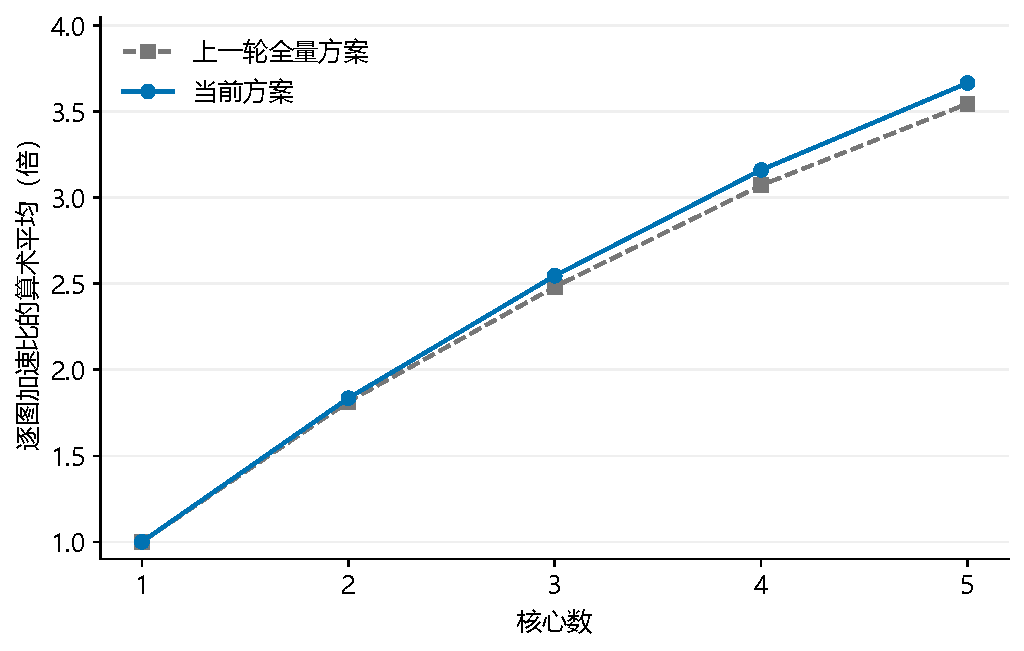
\includegraphics[width=0.85\linewidth,height=0.70\textheight,keepaspectratio]{../图表/fig_q1_r02_mean_speedup.pdf}
\caption{问题一方案一的百图逐图加速比算术平均}\label{fig:q1-speed}
\end{figure}

与本工程上一轮相同百图方案相比，二至五核总周期分别下降 $0.9958\%$、$1.6807\%$、$2.7519\%$、$3.6678\%$；$400$ 个多核配置中 $68$ 胜、$330$ 平、$2$ 负。负例是第 $6$ 图的三核和四核，不能把各阶段收益简单相加，或说每张图都改善。第 $59$ 图在二、四、五核取得本批次最大的逐图加速比，三核最大值来自第 $97$ 图；这些仅为分布端点，不替代百图均值。由于单核分母本身是题目规定的核内启发式而非全局最优，少数多核比值超过核数可以出现，不构成评价错误。

五百份方案均通过官方结构及顺序校验，逐行指标与保存的官方评价相符；代表图还做了冷启动复现。大图采用增量无环检查、状态索引和已固定准备的复用，以减少求解器自身时间；这些工程措施不应被解释成 NPU 任务周期的额外收益。当前热基准搜索最长约 $364$ 秒，但它不含所有配置的冷单核生成和额外最终复核，因此不能断言从零开始每图均在十分钟内结束。完整逐例周期与搬运见附录。
\subsection{平均加速、总周期与执行效率的不同视角}
表\ref{tab:q1-main}中的平均加速比按式\eqref{eq:mean-speedup-derivation}逐图等权统计。为了评价这批图的总体执行负担，表\ref{tab:q1-aggregate-perspective}另把单核总周期 $312\,479\,373$ 作为分母，列出合计周期缩减率与总周期比。数值均直接由同一500行结果表计算，不引入另一批算例。五核总周期较单核下降 $76.5839\%$，其倒数形式的总周期比为 $4.270565$；规定的逐图平均加速比却为 $3.665903$。差异并非评估矛盾，而是式\eqref{eq:weighted-speedup}的权重差异。论文主图仍采用规定的逐图等权均值，总周期比只用于说明大图的绝对时延贡献。
\begin{table}[!htbp]\centering
\caption{问题一结构感知搜索百图总周期视角与逐图等权视角}\label{tab:q1-aggregate-perspective}
\begin{tabular}{rrrrr}
\toprule
核数 & 总周期比 & 总周期下降率 & 平均加速比 & 平均并行效率\\
\midrule
1 & 1.000000 & $0.0000\%$ & 1.000000 & 1.000000\\
2 & 1.968419 & $49.1978\%$ & 1.834917 & 0.917459\\
3 & 2.843802 & $64.8358\%$ & 2.546238 & 0.848746\\
4 & 3.619570 & $72.3724\%$ & 3.161009 & 0.790252\\
5 & 4.270565 & $76.5839\%$ & 3.665903 & 0.733181\\
\bottomrule
\end{tabular}
\end{table}
并行效率定义为 $\eta_k=\overline S_k/k$，只是把相对核数的等权加速程度标准化。五核时 $\eta_5=0.733181$ 并不意味着其余 $26.6819\%$ 的周期都由 DDR 独自造成；关键链、Pipe 不均、释放等待和核内溢出都可能参与。任务执行时间越短是首要目标，不能为了让 $\eta_k$ 的比值好看而故意牺牲 Makespan。后文图\ref{fig:q1-total}的两个子图分别展示逐图平均加速比与百图总周期，报告两个互补视角。


\subsection{典型结果与反例}
第59图的单核参考为 $829\,473$ 周期，五核方案为 $150\,782$ 周期，逐图加速比约 $5.5011$；其额外搬运则从单核 $1\,691\,648$ 增至五核 $4\,325\,376$ 字节。这个例子说明完成时间改善可以伴随更多逻辑搬运，也说明超过五倍的比值并不等于突破硬件计算吞吐上限。赛题的单核分母来自固定的核内启发式，不是单核全局最优；多核切图改变核内问题规模和溢出行为，可能使官方启发式在五核下比把原单核结果简单除以五更有效。第97图单核 $11\,491\,509$、三核 $3\,509\,566$ 周期，加速比约 $3.2743$，是三核配置的分布端点之一。端点代表有利结构，不代表百图平均水平，也不能据此承诺每张图接近理想线性加速。

第6图呈现相反的警示：三核 $32\,925$ 周期、四核 $31\,129$ 周期、五核 $31\,729$ 周期，五核比四核慢。其核数、划分与映射共同改变，不能仅凭这三个总数断言“多一核导致 DDR 拥塞”；需结合时间线中的关键依赖与在途传输核查。该图在前后算法版本比较中三核和四核亦是两处退步，说明有限预算下的新候选机制可能挤掉旧版有价值的候选。故当前选优只保证\emph{同一候选池内}不接受实测变差方案，跨版本必须再做同图同核配置对照。

\subsection{额外搬运与大图求解代价}
二核百图总额外搬运量为 $1\,972\,107\,414$ 字节，高于三核、四核和五核的合计值；五核也略高于四核。这一序列不单调，表明“核数增加必然增加割边搬运”过于简单。算例的实际划分粒度、完整分量分配、共享输入重复读取和核内溢出都随核数变动；如果把所有差值都归咎于跨核边数，便忽略了场景 A 下\emph{同核跨 Task 仍须 DDR}的规则。对本文采用方案，搬运量是次级实测指标，不能由算子数或切边数推算为附录最终值。

大图还有另一种与 NPU 周期不同的成本：主机求解墙钟时间。官方核内启发式、合法性检查和全局事件评估对大型图更贵，若每生成一个局部候选就重新准备全部核内任务，求解过程会浪费大部分时间。对已有结构使用哈希键复用只读准备结果、对商图改变区域增量检查无环，减少的是\emph{找出方案的主机计算}；它不改变候选的官方 $T^A(p)$。本轮100图多核热搜索记录的最长时长约 $363.859$ 秒，含义仅限该阶段；冷启动单核基准和独立最终回放需另外计时。因此本文没有把“每张图端到端5--10分钟”作为已通过的全量实测结论。


\subsection{多候选精修：多结构候选与模拟筛选}
\subsubsection{从图结构形成不同粒度的划分}
单一粒度难以同时处理长链、宽层和大量独立分量。宽层中的细粒度 Task 可以分摊到多个核心，窄层或关键主链若切得过细，却会反复承担 DDR 中转与任务间隔。多候选精修因此构造一组有明确结构依据的划分，而不是只在结构感知搜索所得划分附近作扰动。所有划分仍覆盖每个非 COPY 算子且不重叠，并在加入每核序后检查扩展商图无环。

以原图拓扑层深 $d(v)$ 和层宽 $w_d$ 描述并行结构：
\begin{equation}\label{eq:q1-layer-depth}
d(v)=1+\max_{u\in\operatorname{pred}(v)}d(u),\qquad
w_d=|\{v:d(v)=d\}|,\qquad\max\varnothing=0.
\end{equation}
沿拓扑深度形成粗、细两档窗口；窄层主干采用较粗窗口，宽层及分支采用较细窗口。程序同时枚举若干层宽与深度阈值，保留完整弱连通分量、混合链、按张量字节划分和容量受控批次等候选。主导分量可被拆分，彼此独立的小分量则可按计算 Pipe 负载组合。窗口只是生成合法子图的候选规则，不能由层宽直接推导实际完成时间；被切断的张量还要按共同模型计入中转与等待。

为给任务放置提供较廉价的局部时间尺度，设子图 $r$ 各 Pipe 的估计工作量为 $W_{r,p}$，使用“最长 Pipe 加总工作量补偿”或经核内成本校准的代理：
\begin{equation}\label{eq:q1-allin-proxy}
\widehat\tau_r^{(a)}=\max_p W_{r,p}+0.08\sum_p W_{r,p},\qquad
\widehat\tau_r^{(b)}=\omega\max_p W_{r,p}+(1-\omega)\sum_p W_{r,p}.
\end{equation}
权重 $\omega$ 随候选设置变化，反映 Pipe 重叠程度的不同近似。该式是调度代理，既不宣称是总时长下界，也不以代理最优替代模拟最优。多候选精修保留这些不同代理，是为了在同一真实事件模型下检验它们提出的结构是否有效。

\subsubsection{预计完成时间与后继代价引导的放置}
对每个候选商图，从汇点反向计算任务的后续工作量，以关键任务优先的列表调度构造核心映射。基础放置采用 HEFT 型最早完成时间思想\cite{topcuoglu}：在满足数据释放和同核顺序的可插入位置中选择预计完成较早者。带前瞻的候选还计入后继任务的估计代价，以避免当前任务局部完成较早，却把后继链放到不利的核心。此处的前瞻表仅作排序，跨核释放仍遵循式\eqref{eq:q1-release}，共享 DDR 的最终争用由官方事件模拟计算。

与结构感知搜索的单个配置最多 $12$ 次完整评价不同，多候选精修先保留基础候选，再追加结构层候选，按划分、映射和顺序的规范指纹去重。其五核扩展包括额外层结构及局部搜索；这些设置不能直接当成一至四核均已验证的算法收益。设候选集合为 $\mathcal C_0$，模拟阶段求
\begin{equation}\label{eq:q1-allin-choice}
p_0=\arg\min_{p\in\mathcal C_0\cap\mathcal P_A(k)}
\operatorname{lex}\bigl(T_i^A(p),D_i(p)\bigr).
\end{equation}
由于 $\mathcal C_0$ 并不保证包含结构感知搜索的最终解，多候选精修不存在逐图必优保证；即使百图均值提高，仍需检查逐图退步。

\subsubsection{五核局部改进与算法步骤}
五核局部搜索以已评价最优方案为起点，保持子图划分，尝试核心迁移、交换和保持拓扑合法的核心顺序调整。若修改不满足覆盖或无环条件，直接拒绝；若官方模拟的字典序目标不改善，不替换当前最优。局部步数随图规模递减，超过 $9000$ 个计算操作时跳过该扩展，以限制大图代价。历史运行设置了局部阶段 $600$ 秒墙钟界限，并以已发生的构造评价成本决定是否进入局部搜索；这不是整个冷启动流程的 $600$ 秒保证。

算法的完整步骤如下。
\begin{enumerate}
\item 读取图及硬件配置，计算拓扑层、弱连通分量、主链、Pipe 工作量与共享张量关系。
\item 生成完整分量、粗细窗口、混合链和容量批次等划分，分别用基础及带前瞻的列表调度映射到核心。
\item 去除重复与非法候选，逐一调用官方内层排程与共享 DDR 事件模拟，按式\eqref{eq:q1-allin-choice}保存实测最优。
\item 五核配置在规模和时间条件允许时，对固定划分执行迁核、交换与顺序邻域搜索，更新实测最优。
\item 输出子图归属与每核顺序；独立恢复并回放保存的方案，核对周期和额外搬运，不把恢复历史方案的时间作为全新搜索时间。
\end{enumerate}
记结构候选数为 $M$，局部提案数为 $L$，一次构造、合法性检查和官方评价成本分别为 $C_g,C_v,C_e$，则总成本可写为
\begin{equation}\label{eq:q1-allin-complexity}
O\bigl(M(C_g+C_v+C_e)+L(C_v+C_e)\bigr).
\end{equation}
固定候选的商图无环检查为 $O(q+|E_\pi|)$；$C_e$ 还受核内准备、溢出和在途事件数量影响，不能笼统写成只依赖节点数的常数。因此多候选精修的主要代价来自更丰富的候选及相应模拟，并未消除大图评价瓶颈。

\subsection{两种方案的比较与适用范围}
\subsubsection{完整核数曲线}
多候选精修的一至四核补跑及独立复核已完成，现与五核已核实组合共同组成100图、1至5核的500组结果。图\ref{fig:q1-complete}将两方法按相同算例及固定单核分母对齐。多候选精修的五点平均加速比分别为1.000000、1.860204、2.604827、3.272613和4.026824；多核均值均高于结构感知搜索，但三核总周期为110359308，高于后者的109880862。说明逐图等权的平均收益不能替代整批图的周期比较。五核沿用已恢复核对的交付组合，低核采用本次补跑结果；本图不构成全部配置等预算重新搜索的实验。

\begin{figure}[!htbp]\centering
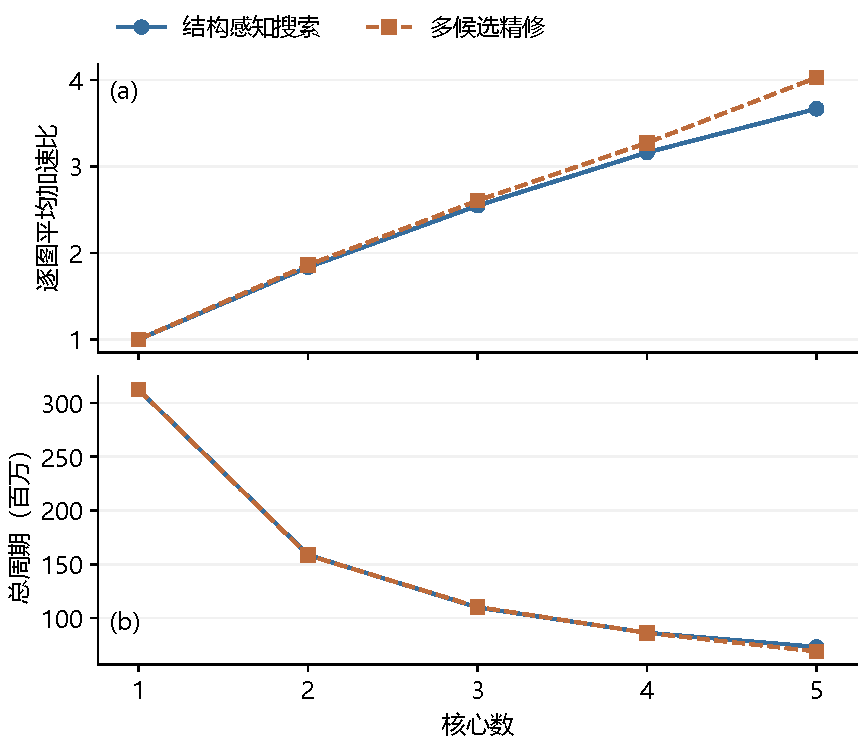
\includegraphics[width=0.92\linewidth,height=0.70\textheight,keepaspectratio]{../图表/runs/20260926-A-six-figures/fig_q1_complete_curves.pdf}
\caption{两种方法在100图、1至5核下的平均加速比与总周期}\label{fig:q1-complete}\label{fig:q1-speed}\label{fig:q1-total}
\end{figure}
\subsubsection{相同单核分母下的五核结果}
采用相同的 $100$ 张输入图及同一官方评价语义，将两种方案逐图配对。结构感知搜索取已交付的 r02 结果；多候选精修取 Allin2 最新交付组合，并恢复全部 $100$ 份五核方案作官方回放。两批逐图单核分母逐项一致，恢复结果的完成周期及额外搬运均与保存的交付摘要一致。该核对支持输出结果比较，不代表重新实施了等预算的算法实验。
\begin{table}[!htbp]\centering
\caption{问题一两种方案的百图五核配对比较}\label{tab:q1-two-methods}
\begin{tabular}{lrr}
\toprule
指标 & 结构感知搜索 & 多候选精修\\
\midrule
逐图平均加速比 & 3.665903 & 4.026824\\
总完成周期（cycles） & 73170501 & 68905422\\
总额外搬运（bytes） & 1767728284 & 1807542424\\
配对图数 & 100 & 100\\
\bottomrule
\end{tabular}
\end{table}
多候选精修相对结构感知搜索为 66 胜、21 平、13 负，胜负按完成周期判断。平均加速比相对提高 9.85\%，总完成周期下降 5.83\%。前一指标对每图等权，后一指标更受大图影响，二者不可互换；多候选精修的总额外搬运反而增加约 2.25\%，表明其周期收益并非来自总搬运量的整体减少，而与并行安排及关键等待有关。搬运作为次级指标单列，不替代完成周期。

图\ref{fig:q1-case-gains}按五核逐图周期改善率从小到大排列全部100个算例，改善率定义为“结构感知搜索周期减多候选精修周期”，再除以结构感知搜索周期。横轴是排序位置而非原始算例编号，负值完整保留。多数改善集中于一部分图，仍有13个退步例，故不能把平均改善解释为逐图支配。

\begin{figure}[!htbp]\centering
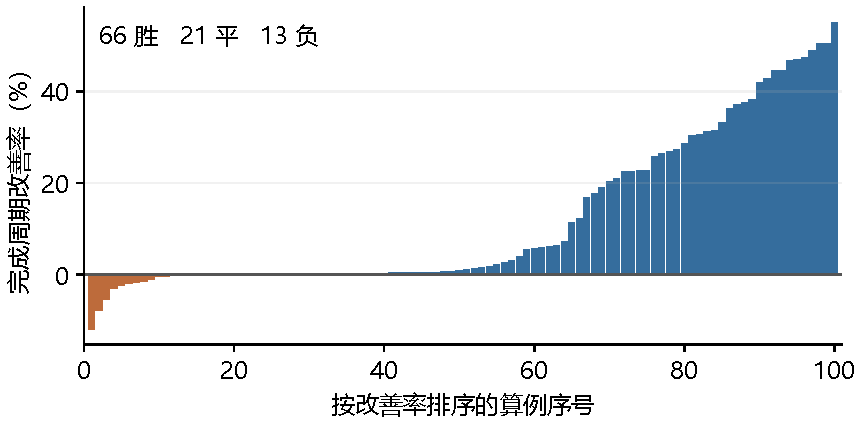
\includegraphics[width=0.92\linewidth,height=0.70\textheight,keepaspectratio]{../图表/runs/20260926-A-six-figures/fig_q1_case_gains.pdf}
\caption{五核逐图完成周期改善率分布}\label{fig:q1-case-gains}
\end{figure}
\subsubsection{性能收益与计算预算的边界}
结构感知搜索把评价机会限制为 $12$，适合昂贵模拟条件下的稳定基线。多候选精修覆盖更多层结构和映射候选，能改善整体五核结果，但历史全量搜索平均约 $708.98$ 秒、最长约 $3371.6$ 秒，$49$ 张图的搜索评价时间超过 $600$ 秒。这些历史统计来自全量搜索记录，并非本次恢复过程或最新交付组合的端到端计时；交付摘要还组合了不同阶段的已得方案。因此，当前对照能说明最终交付质量差异，不能单独归因于变宽划分、前瞻放置或局部搜索中的某一项。

若硬性限制在线求解资源，宜先采用结构感知搜索作为可复核基线，再在统一评价次数与统一墙钟预算下比较多候选精修。若允许离线充分搜索，可采用多候选精修已核实的五核组合。一至四核结果现已独立复核并纳入完整核数曲线，但仍需等预算消融和端到端计时，才能判断不同机制的独立收益。两种方案均为有限候选启发式，未证明全局最优。


